% ============================================================
% P1-REPORT.tex -- Final Project Report
% AI-Based Customer Segmentation and Personalized WhatsApp Marketing Platform
% ============================================================
\documentclass[12pt,a4paper]{report}

\usepackage[T1]{fontenc}
\usepackage[utf8]{inputenc}
\usepackage{mathptmx}
\usepackage{amsmath,amssymb,amsfonts}
\usepackage{setspace}
\usepackage{fancybox}
\usepackage{pdfpages}
\usepackage{hyperref}
\usepackage{cite}
\usepackage{fancyhdr}
\usepackage{array}
\usepackage{booktabs}
\usepackage{longtable}
\usepackage{enumitem}
\usepackage{graphicx}
\usepackage[font=small,labelfont=bf]{caption}
\usepackage{xcolor}
\usepackage{indentfirst}
\usepackage{titlesec}
\usepackage{multirow}
\usepackage{tabularx}
\usepackage{float}
\usepackage{listings}
\usepackage{tikz}
\usetikzlibrary{arrows.meta,fit,positioning,shapes.geometric}
\usepackage[a4paper,top=25.4mm,bottom=32mm,left=37mm,right=25.4mm]{geometry}

\onehalfspacing
\setlength{\parindent}{2em}
\setlength{\parskip}{6pt}
\setlist{itemsep=3pt,topsep=4pt}

\makeatletter
\def\@makechapterhead#1{%
  \vspace*{5\p@}%
  {\parindent \z@ \centering \normalfont
    \ifnum \c@secnumdepth >\m@ne
      \fontsize{14}{16}\selectfont\bfseries \thechapter.\space
    \fi
    \interlinepenalty\@M
    \fontsize{14}{16}\selectfont\bfseries\MakeUppercase{#1}\par\nobreak
    \vskip 10\p@
  }}
\makeatother

\titleformat{\section}{\bfseries\fontsize{12}{14}\selectfont}{\thesection}{0.5em}{\MakeUppercase}
\titlespacing*{\section}{0pt}{14pt}{6pt}
\titleformat{\subsection}{\bfseries\fontsize{12}{14}\selectfont}{\thesubsection}{0.5em}{}
\titlespacing*{\subsection}{0pt}{10pt}{4pt}
\titleformat{\subsubsection}{\fontsize{12}{14}\selectfont}{\thesubsubsection}{0.5em}{}
\titlespacing*{\subsubsection}{0pt}{8pt}{4pt}

\hypersetup{colorlinks=true,linkcolor=black,citecolor=black,urlcolor=black,pdftitle={AI-Based Customer Segmentation and Personalized WhatsApp Marketing Platform}}
\lstset{basicstyle=\ttfamily\small,breaklines=true,frame=single,columns=fullflexible}

\pagestyle{fancy}
\fancyhf{}
\renewcommand{\headrulewidth}{0.4pt}
\renewcommand{\footrulewidth}{0.4pt}
\fancyhead[C]{\fontsize{10}{12}\selectfont\textrm{AI-BASED CUSTOMER SEGMENTATION AND PERSONALIZED WHATSAPP MARKETING PLATFORM}}
\fancyfoot[C]{\fontsize{10}{12}\selectfont\textrm{PICT - INFORMATION TECHNOLOGY -- 2024-25}}
\fancyfoot[R]{\fontsize{10}{12}\selectfont\textrm{\thepage}}
\fancypagestyle{plain}{\fancyhf{}\renewcommand{\headrulewidth}{0.4pt}\renewcommand{\footrulewidth}{0.4pt}\fancyhead[C]{\fontsize{10}{12}\selectfont\textrm{AI-BASED CUSTOMER SEGMENTATION AND PERSONALIZED WHATSAPP MARKETING PLATFORM}}\fancyfoot[C]{\fontsize{10}{12}\selectfont\textrm{PICT - INFORMATION TECHNOLOGY -- 2024-25}}\fancyfoot[R]{\fontsize{10}{12}\selectfont\textrm{\thepage}}}

\newcommand{\projecttitle}{AI-Based Customer Segmentation and Personalized WhatsApp Marketing Platform}
\newcommand{\placeholder}[1]{\textit{[#1]}}
\newcommand{\guidename}{Mr.~Sandeep R.~Warhade}

\begin{document}

% ------------------------------------------------------------
% Front matter
% ------------------------------------------------------------
\pagenumbering{gobble}
\thispagestyle{empty}
\setlength{\unitlength}{1in}
\begin{picture}(0,0)
  \put(-0.45,-10.25){\framebox(6.7,10.2){}}
\end{picture}
\begin{center}
\vspace*{0.12in}
\textbf{\large A PRELIMINARY PROJECT REPORT}

\vspace{0.08in}
ON

\vspace{0.22in}
\textbf{\LARGE AI-BASED CUSTOMER SEGMENTATION AND\\[6pt] PERSONALIZED WHATSAPP MARKETING PLATFORM}

\vspace{0.22in}
Submitted to the Savitribai Phule Pune University, Pune\\
in partial fulfillment of the requirements for the award of the degree of

\vspace{0.16in}
\textbf{\Large Bachelor of Engineering in Information Technology}

\vspace{0.22in}
\textbf{\large BY}

\vspace{0.12in}
\begin{tabular}{c c}
\textbf{Sushant Bhanwase} & \textbf{43106}\\[3pt]
\textbf{Sarthak Gawari} & \textbf{43133}\\[3pt]
\textbf{Yash Kachale} & \textbf{43323}\\[3pt]
\textbf{Jaykumar Kale} & \textbf{43324}
\end{tabular}

\vspace{0.2in}
\textbf{\large UNDER THE GUIDANCE OF}\\[6pt]
\guidename

\vspace{0.2in}

\includegraphics[width=1.15in]{pict_logo.png}

\vspace{0.12in}
\textbf{\large DEPARTMENT OF INFORMATION TECHNOLOGY}\\
\textbf{PUNE INSTITUTE OF COMPUTER TECHNOLOGY, PUNE -- 411\,043}\\
\textbf{2026--2027}
\end{center}

\newpage
\pagenumbering{roman}
\setcounter{page}{1}
\thispagestyle{empty}
\setlength{\unitlength}{1in}
\begin{picture}(0,0)
  \put(-0.45,-9.65){\framebox(6.7,9.6){}}
\end{picture}
\begin{center}
\textbf{\large SCTR's}\\
\textbf{\large PUNE INSTITUTE OF COMPUTER TECHNOLOGY}\\
\textbf{DEPARTMENT OF INFORMATION TECHNOLOGY}

\vspace{0.3in}

\includegraphics[width=1.15in]{pict_logo.png}

\vspace{0.3in}
\textbf{\LARGE \underline{C E R T I F I C A T E}}
\end{center}

\vspace{0.25in}
This is to certify that the project report entitled
\begin{center}\textbf{\projecttitle}\end{center}
submitted by
\begin{center}
\begin{tabular}{c c}
\textbf{Sushant Bhanwase} & \textbf{43106}\\
\textbf{Sarthak Gawari} & \textbf{43133}\\
\textbf{Yash Kachale} & \textbf{43323}\\
\textbf{Jaykumar Kale} & \textbf{43324}
\end{tabular}
\end{center}
is a bonafide work carried out under the supervision of \guidename. The work is submitted in partial fulfillment of the requirements of Savitribai Phule Pune University for the award of the degree of Bachelor of Engineering in Information Technology.

\vspace{0.6in}
\begin{tabular}{p{2.8in}p{2.8in}}
\textbf{\guidename} & \textbf{Dr. S. C. Dharmadhikari}\\
Internal Project Guide & Head, Department of Information Technology\\[24pt]
\textbf{\placeholder{External Examiner}} & \textbf{Dr. S. T. Gandhe}\\
External Examiner & Principal, PICT Pune
\end{tabular}

\vspace{0.5in}
Date: \underline{\hspace{1.5in}} \hspace{1in} Place: Pune

\newpage
\thispagestyle{plain}
\begin{center}\textbf{\LARGE DECLARATION}\end{center}
\addcontentsline{toc}{section}{Declaration}
We declare that the project report entitled \textbf{\projecttitle} is our original work carried out as part of the Bachelor of Engineering programme in Information Technology. The implementation, experiments, documentation, and analysis presented in this report were completed for the project repository identified in this work.

The report distinguishes verified results of the implemented batch MVP from proposed real-time research extensions. The synthetic verification dataset, source code, tests, and generated project outputs are cited where they support a claim. No result from an unimplemented event-driven system is presented as an achieved result.

\vspace{0.7in}
\begin{flushright}
\begin{tabular}{c c}
\textbf{Sushant Bhanwase} & \textbf{43106}\\[12pt]
\textbf{Sarthak Gawari} & \textbf{43133}\\[12pt]
\textbf{Yash Kachale} & \textbf{43323}\\[12pt]
\textbf{Jaykumar Kale} & \textbf{43324}
\end{tabular}
\end{flushright}

\newpage
\thispagestyle{plain}
\begin{center}\textbf{\LARGE ACKNOWLEDGEMENT}\end{center}
\addcontentsline{toc}{section}{Acknowledgement}
We express our sincere gratitude to our project guide, \guidename, for technical direction, constructive review, and encouragement throughout the project. The feedback received during planning, implementation, and evaluation helped us convert an initial marketing idea into a reproducible software system.

We thank Dr. S. C. Dharmadhikari, Head of the Department of Information Technology, and Dr. S. T. Gandhe, Principal, Pune Institute of Computer Technology, for providing the academic environment and infrastructure required for this work.

We acknowledge the foundational contributions of Hughes, MacQueen, Rousseeuw, Davies and Bouldin, Calinski and Harabasz, and other researchers whose work informs RFM analysis, clustering, and customer analytics. We also thank our families and colleagues for their patience and support during the development and testing of the platform.

\vspace{1.2in}
\begin{flushright}
\begin{tabular}{c c}
Sushant Bhanwase & 43106\\[12pt]
Sarthak Gawari & 43133\\[12pt]
Yash Kachale & 43323\\[12pt]
Jaykumar Kale & 43324
\end{tabular}
\end{flushright}

\newpage
\thispagestyle{plain}
\listoffigures
\addcontentsline{toc}{section}{List of Figures}

\newpage
\thispagestyle{plain}
\listoftables
\addcontentsline{toc}{section}{List of Tables}

\newpage
\thispagestyle{plain}
\begin{center}\textbf{\LARGE ABBREVIATIONS}\end{center}
\addcontentsline{toc}{section}{Abbreviations}
\begin{longtable}{l @{\hspace{0.35in}:\hspace{0.25in}} p{4.4in}}
API & Application Programming Interface\\
CSV & Comma-Separated Values\\
DBI & Davies--Bouldin Index\\
DPDP & Digital Personal Data Protection\\
GDPR & General Data Protection Regulation\\
HTTP & Hypertext Transfer Protocol\\
JSON & JavaScript Object Notation\\
K-Means & K-Means clustering algorithm\\
ML & Machine Learning\\
ORM & Object-Relational Mapping\\
RFM & Recency, Frequency, Monetary\\
REST & Representational State Transfer\\
SQL & Structured Query Language\\
UCD & Use Case Diagram\\
UI & User Interface\\
WCSS & Within-Cluster Sum of Squares\\
XAI & Explainable Artificial Intelligence
\end{longtable}

\newpage
\thispagestyle{empty}
\addcontentsline{toc}{section}{Contents}
\tableofcontents

\newpage
\thispagestyle{plain}
\begin{center}\textbf{\fontsize{12}{14}\selectfont ABSTRACT}\end{center}
\addcontentsline{toc}{section}{Abstract}
This project presents a platform for customer segmentation and consent-aware WhatsApp campaign recommendation. The batch workflow validates transaction CSV files, isolates cancellations and duplicates, calculates customer-level Recency, Frequency, and Monetary (RFM) features, evaluates K-Means models, creates interpretable segment labels, and applies consent, suppression, recency, and rolling frequency-cap checks. On the bundled synthetic dataset, 57 raw rows represent 15 customers; 52 rows are retained, two cancellations are isolated, five rows are dropped, and one duplicate is removed. With random seed 42, the selected model has $K=3$, silhouette score 0.4562, Davies--Bouldin index 0.7150, and Calinski--Harabasz score 13.42. Twelve customers are approved and three are blocked by policy rules. The FastAPI and React MVP is tested by 87 passing tests. Real-time event processing and live WhatsApp dispatch remain future work.

\vspace{0.12in}
\noindent\textbf{Keywords:} Customer segmentation, RFM analysis, K-Means clustering, marketing fatigue, consent-aware recommendation, WhatsApp, FastAPI, React.

% ------------------------------------------------------------
\clearpage\pagenumbering{arabic}
\chapter{Introduction}
\section{Background}
Digital commerce systems generate large volumes of transaction records. Each record usually describes an invoice, a customer, a date, a quantity, and a unit price. The information is valuable because it reveals behavioural patterns, but it is difficult to use directly when a marketing team needs a concise answer to three questions: which customers are valuable, which customers are becoming inactive, and which customers can be contacted responsibly?

A common operational response is to send the same message to a broad audience. This approach is simple but ignores differences in purchase behaviour and can create marketing fatigue. It also creates a governance problem: a customer may have withdrawn consent, may be on a suppression list, or may already have received the maximum number of messages allowed in a rolling period. A useful system therefore has to combine behavioural analysis with explicit communication constraints.

This project develops a platform that addresses this combined problem. The analytical core uses RFM features and unsupervised clustering. The decision layer maps interpretable customer groups to campaign archetypes. The governance layer prevents an otherwise attractive recommendation from becoming an unauthorised outreach decision. The user interface exposes the process as a sequence of upload, analysis, segments, metrics, and recommendations views.

\section{Motivation}
RFM analysis is attractive for a project implementation because it is understandable to both technical and business audiences. Recency measures how recently a customer purchased, frequency measures repeated purchasing, and monetary value measures the amount spent. Together they form a compact behavioural representation without requiring personally intrusive attributes.

Clustering is useful when labelled outcomes are unavailable. A business may not have enough reliable historical campaign-response labels to train a supervised model. K-Means can still identify groups with similar behaviour, provided that data quality, scaling, cluster selection, and interpretation are documented. The resulting labels are descriptive rather than predictive.

WhatsApp is treated in this project as a delivery channel and preview surface, not as permission to contact customers automatically. The system uses a mock adapter by default. This protects development and demonstration environments from accidental dispatch and makes the difference between a recommendation, a preview, and a delivered message explicit.

\section{Problem Statement}
Transaction data is frequently stored as a collection of uncleaned line items. Missing identifiers, invalid dates, cancellations, negative quantities, duplicate lines, and extreme monetary values can distort customer profiles. Even after cleaning, unsupervised clusters do not automatically translate into safe campaign decisions. A system is required that performs the following operations in a traceable order:
\begin{enumerate}
\item validate and clean transaction data;
\item construct customer-level RFM features;
\item select and explain a clustering configuration;
\item produce data-driven customer segment labels;
\item recommend a campaign archetype with supporting reasons; and
\item block recommendations that violate consent, suppression, or fatigue rules.
\end{enumerate}

\section{Research Question}
The implemented project answers the engineering question: \emph{Can a reproducible RFM and K-Means workflow provide explainable customer segments and policy-aware campaign recommendations through a usable web dashboard?}

The related future research question is: \emph{Can a stability-aware decision layer improve real-time RFM updates while maintaining low latency and eligibility guarantees?} The second question is not claimed as answered because the event-driven extension has not been implemented or evaluated.

\section{Objectives}
The objectives of the completed project are:
\begin{enumerate}
\item Build a robust CSV ingestion and quality-control pipeline.
\item Calculate RFM features using clear business definitions.
\item Evaluate K-Means values of $K$ using three internal metrics.
\item Generate dynamic segment labels from cluster statistics.
\item Implement explainable campaign recommendations.
\item Enforce consent, suppression, and rolling frequency-cap rules.
\item Provide REST endpoints for analysis and a connected React dashboard.
\item Provide a mock-by-default WhatsApp adapter and preview workflow.
\item Verify core services using automated tests.
\end{enumerate}

\section{Scope}
The scope includes batch CSV ingestion, customer-level analytics, unsupervised segmentation, deterministic recommendations, policy checks, API endpoints, dashboard views, and component testing. The scope does not include production authentication, a complete multi-tenant API workflow, durable event queues, a public WhatsApp webhook, live message dispatch, or a claim of campaign conversion improvement.

\section{Report Organization}
Chapter 1 introduces the problem and scope. Chapter 2 discusses the domain and relevant technical background. Chapter 3 presents requirements and feasibility. Chapter 4 describes the system architecture. Chapter 5 explains the data pipeline and RFM feature engineering. Chapter 6 presents clustering and recommendation methodology. Chapter 7 covers implementation. Chapter 8 describes the dashboard and user workflow. Chapter 9 reports testing and verified results. Chapter 10 discusses security, privacy, ethics, and limitations. Chapter 11 presents deployment and operation. Chapter 12 concludes the completed work and identifies future research.

\chapter{Literature Review and Technical Background}
\section{Customer Relationship Management}
Customer relationship management systems collect interactions and transactions so that an organisation can understand customer needs and coordinate communication. A transaction record is useful for operational accounting, but a marketing decision requires derived features. The platform therefore treats raw records as evidence from which an auditable profile is calculated.

A segmentation system can support prioritisation, but segmentation is not equivalent to personal knowledge. A cluster describes similarity under the selected features and preprocessing choices. It does not explain a customer's motives, demographic identity, or future response. This distinction is maintained in the project by using descriptive labels and heuristic campaign scores rather than claiming a predicted probability of conversion.

\section{RFM Analysis}
RFM is a widely used behavioural framework for direct marketing \cite{hughes1994,chen2012}. For a customer $i$, recency is the elapsed time since the most recent valid purchase, frequency is the number of distinct invoices, and monetary value is the sum of valid line totals. The measures are compact, explainable, and suitable for small datasets.

RFM is not automatically reliable. The reference date must be defined, cancellation rows must not inflate spend, duplicate records must not inflate frequency, and skewed monetary values can dominate distance-based clustering. The project makes each of these choices explicit.

\section{Unsupervised Clustering}
K-Means partitions feature vectors into $K$ groups by repeatedly assigning each vector to its nearest centroid and updating centroids \cite{macqueen1967}. Its objective function is:
\begin{equation}
J = \sum_{k=1}^{K}\sum_{x_i\in S_k}\lVert x_i-\mu_k\rVert^2,
\end{equation}
where $S_k$ is cluster $k$ and $\mu_k$ is its centroid. K-Means is computationally practical, but the result depends on feature scale, the selected $K$, initialisation, and random seed.

The project reports silhouette, Davies--Bouldin, and Calinski--Harabasz indices \cite{rousseeuw1987,davies1979,calinski1974}. The silhouette score compares cohesion with separation and is maximised. The Davies--Bouldin index measures similarity to the most similar competing cluster and is minimised. The Calinski--Harabasz score compares between-cluster dispersion with within-cluster dispersion and is maximised. No single score is treated as proof of business value.

\section{Marketing Fatigue and Consent}
A recommendation should not override a customer's communication preferences. The implemented fatigue service applies hard checks: explicit consent must be true, suppression must be false, and the number of messages in the last 30 days must remain below the configured cap. Campaign-specific recency rules may additionally affect eligibility. The output includes both passed and failed checks so that a marketer can inspect the reason.

The default frequency cap is three messages in a rolling 30-day window. Contact fatigue and coordinated multichannel communication are established concerns in customer relationship management \cite{godfrey2011,kumar2016,verhoef2015}. This is a project policy parameter, not a universal legal threshold. In production, the parameter would require organisational approval, regulatory review, and monitoring.

\section{Explainable Artificial Intelligence}
Explainability in this project means that each recommendation includes the segment label, RFM values, campaign type, heuristic priority score, policy status, and a natural-language rationale. The system does not claim that this explanation is a causal explanation. It is an audit-oriented description of the deterministic rules that produced the recommendation.

\section{Messaging Integration}
The WhatsApp integration follows an adapter design. A mock adapter returns a simulated message result for development. A live adapter skeleton can be configured only when explicit credentials and live-mode configuration are supplied. The project demonstration remains simulated. A preview is not a delivery receipt, and a recommendation is not a permission grant.

\chapter{Requirement Specification and Analysis}
\section{Functional Requirements}
\begin{longtable}{p{0.15\textwidth}p{0.72\textwidth}}
\caption{Functional requirements}\label{tab:functional}\\
\toprule
ID & Requirement\\\midrule
FR1 & The system shall accept a transaction CSV through the upload endpoint.\\
FR2 & The system shall validate required columns and common header aliases.\\
FR3 & The system shall report rejected rows, cancellations, and duplicates.\\
FR4 & The system shall calculate customer-level recency, frequency, and monetary values.\\
FR5 & The system shall evaluate feasible K-Means cluster counts and report metrics.\\
FR6 & The system shall generate descriptive labels from cluster statistics.\\
FR7 & The system shall expose segment profiles and customer RFM results.\\
FR8 & The system shall produce a campaign recommendation with supporting explanation.\\
FR9 & The system shall block outreach when consent, suppression, or fatigue checks fail.\\
FR10 & The system shall provide a simulated WhatsApp preview without live dispatch by default.\\
FR11 & The dashboard shall display ingestion, metrics, segments, and recommendations.\\
FR12 & The test suite shall cover the core services and policy boundaries.\\\bottomrule
\end{longtable}

\section{Non-Functional Requirements}
The system should be reproducible with a fixed seed and documented input. It should provide understandable error messages, separate computation from presentation, avoid leaking secrets into source files, and preserve a safe default for messaging. The API should return structured JSON responses and the dashboard should remain usable when the backend is unavailable by displaying a health status rather than silently presenting stale results.

\section{Use Cases}
The primary actor is a marketing analyst. The analyst uploads a CSV, reviews data-quality findings, runs analysis, inspects cluster metrics, examines segment profiles, filters recommendations, and opens a simulated message preview. A system administrator configures the environment and controls whether live mode is available. A future integration actor would submit transaction or delivery events, but that use case is outside the completed MVP.

\begin{table}[H]
\centering
\caption{Primary use-case flow}
\label{tab:usecase}
\begin{tabular}{p{0.24\textwidth}p{0.62\textwidth}}
\toprule
Use case & Main flow\\\midrule
Upload data & Select file, send to API, display validation summary.\\
Run analysis & Start RFM and clustering, store process-local result.\\
Inspect segments & View segment size, medians, labels, and customer profiles.\\
Review recommendations & View campaign type, score, explanation, and policy checks.\\
Preview campaign & Open simulated WhatsApp message for an eligible customer.\\
Review health & Poll the API health endpoint and show service state.\\\bottomrule
\end{tabular}
\end{table}

\section{Feasibility Analysis}
\subsection{Technical Feasibility}
The project is technically feasible because the workload is small enough for pandas and scikit-learn, while FastAPI provides a clear service boundary. React and TypeScript provide a typed browser client without requiring a large frontend framework. The architecture leaves room for SQLite during development and PostgreSQL in a later deployment.

\subsection{Operational Feasibility}
The dashboard follows the analyst's natural workflow: data first, analysis second, interpretation third, and action last. The mock adapter reduces operational risk during demonstrations. Explanations and failed policy checks support review by users who may not inspect Python source code.

\subsection{Economic Feasibility}
The implementation uses open-source software and local development tools. A production deployment would introduce costs for hosting, database operations, observability, and WhatsApp Business API usage. Those costs are outside the completed local MVP.

\subsection{Legal and Ethical Feasibility}
The system is designed around consent and suppression checks. The bundled dataset is synthetic and uses customer identifiers such as `CUST001`; no real phone numbers are required. A production system would need an approved lawful basis, retention policy, access control, and review of applicable privacy and messaging regulations.

\chapter{System Analysis and Design}
\section{Architecture Overview}
The active application contains a React frontend, a FastAPI backend, analytical services, policy services, and a mock messaging adapter. The current upload and analysis workflow is process-local through `backend/session.py`. SQLAlchemy models and tenant helpers exist in the repository, but they are not wired into every active router. This distinction is important because the report describes what runs today rather than an intended production architecture.

\begin{figure}[H]
\centering
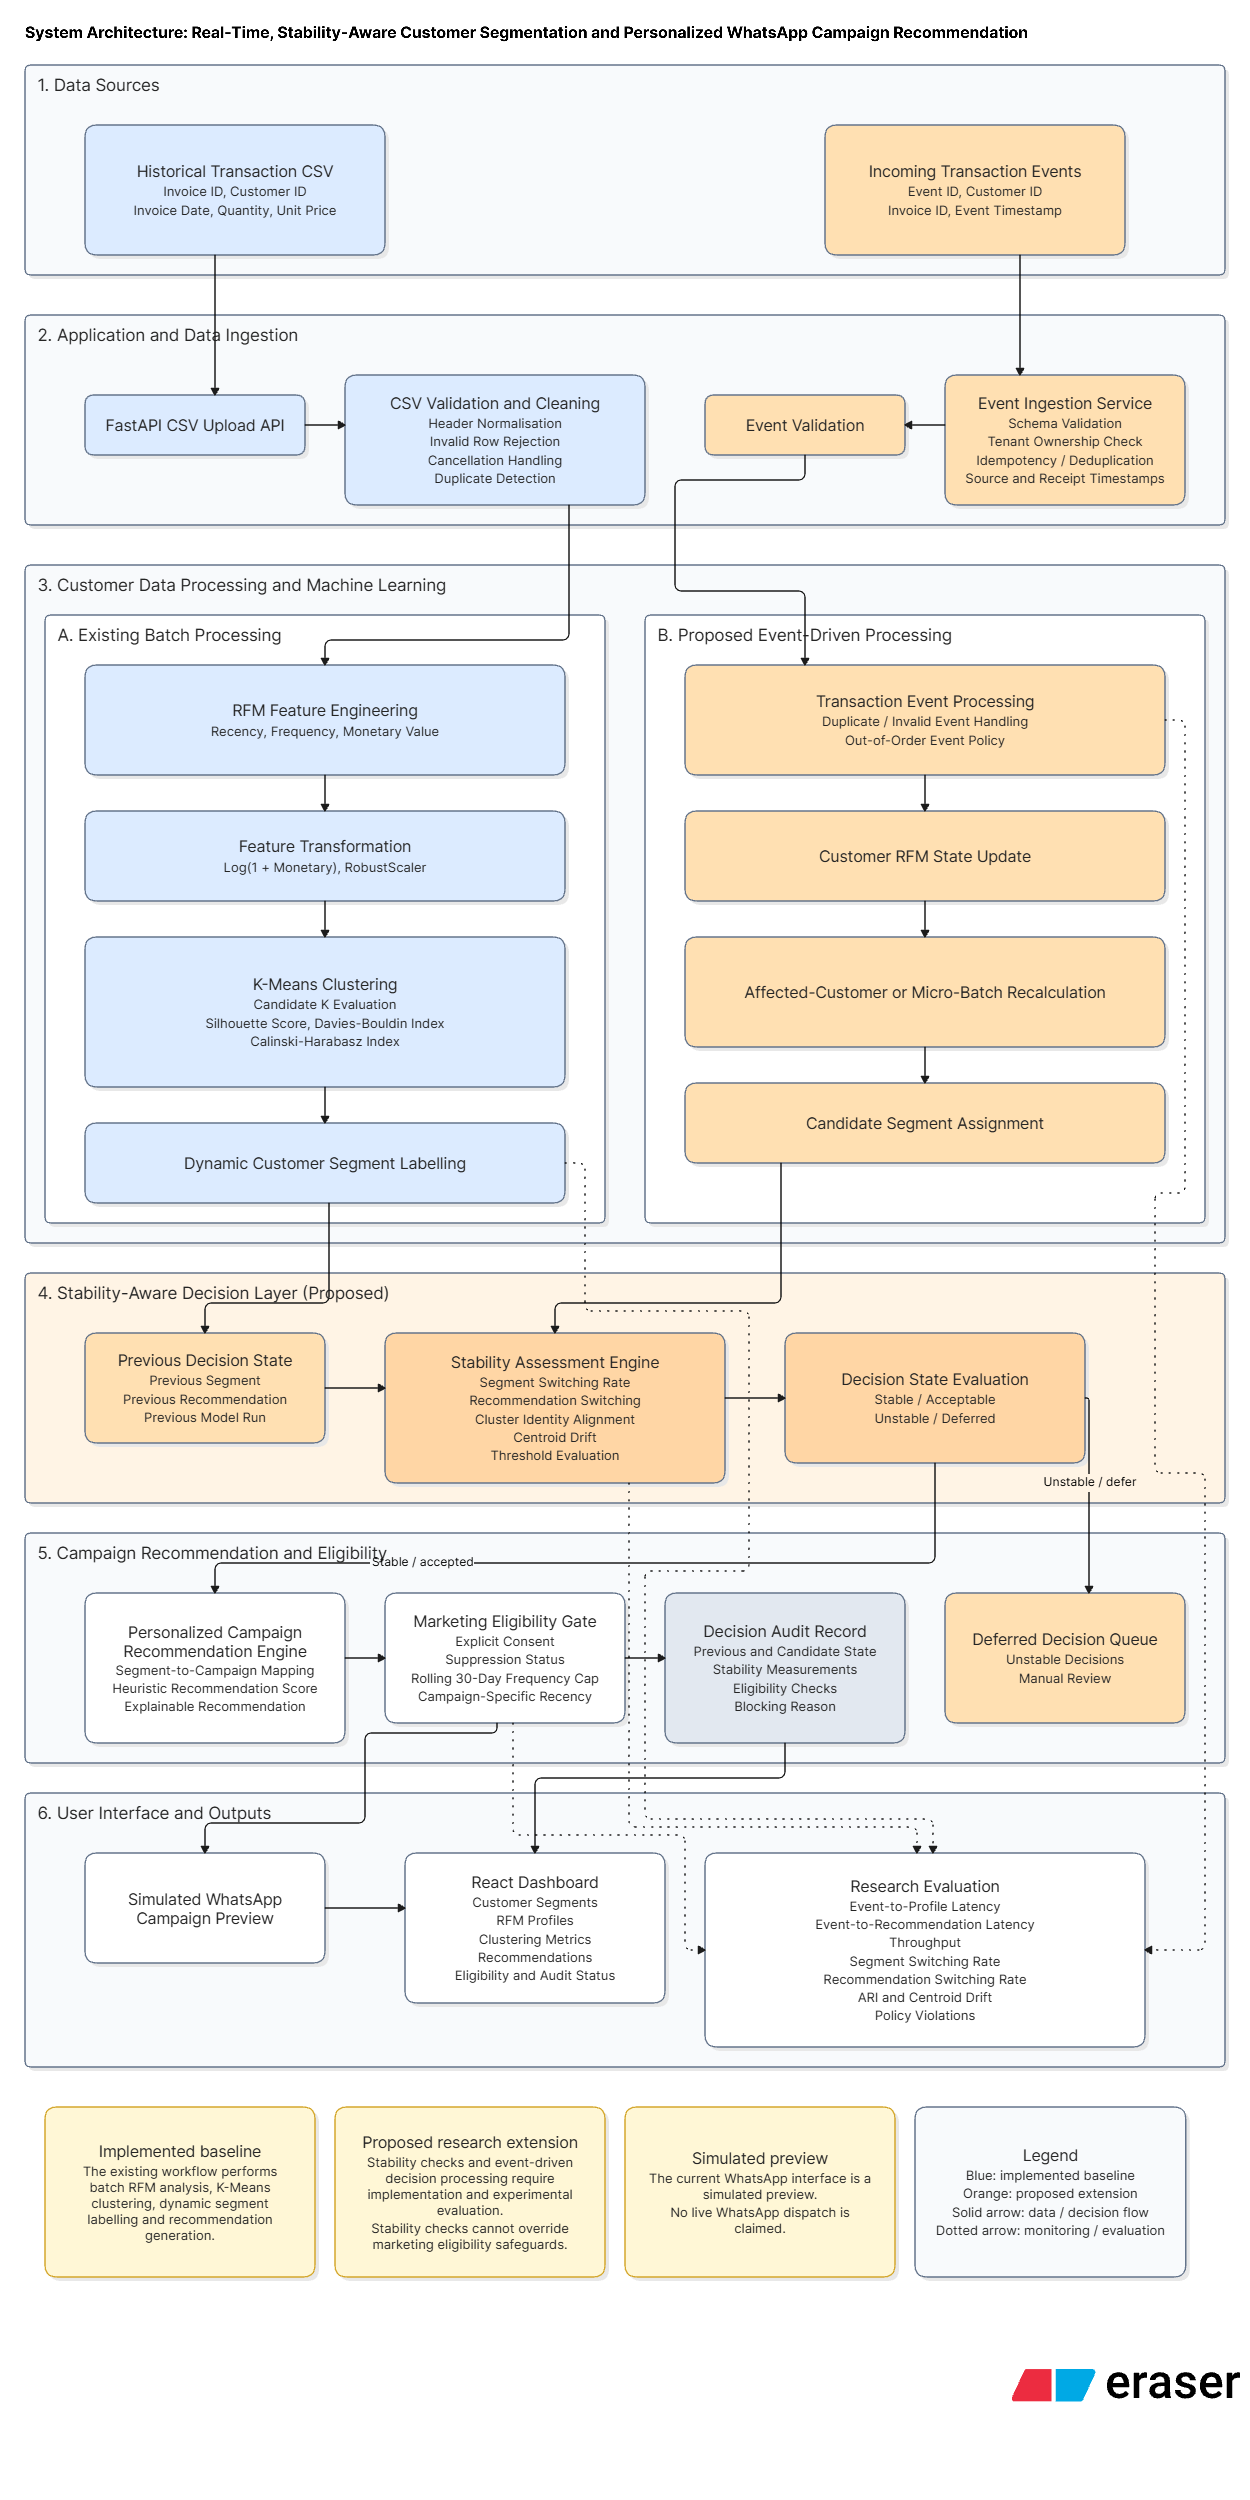
\includegraphics[width=\textwidth,height=0.78\textheight,keepaspectratio,trim=0 180 0 0,clip]{Stability-Aware Customer Segmentation Architecture.png}
\caption{System Architecture: Real-Time, Stability-Aware Customer Segmentation and Personalized WhatsApp Campaign Recommendation. Blue denotes the implemented batch baseline; orange denotes the proposed extension.}
\label{fig:architecture}
\end{figure}

\section{Backend Modules}
The `main.py` entry point creates the FastAPI application, configures CORS from environment settings, and registers the active routers. The health router provides a service status response. The ingestion router accepts uploaded data and returns a cleaning summary. The analysis router executes RFM and clustering. Segment and recommendation routers expose computed results to the frontend.

The service layer keeps domain operations separate. The ingestion service is responsible for normalisation and validation. The RFM service aggregates customer features and assigns ordinal scores. The clustering service transforms features, evaluates K values, and creates dynamic labels. The fatigue service applies eligibility rules. The recommendation service combines segment characteristics with policy output.

\section{Frontend Modules}
The frontend is a React 18 and TypeScript application built with Vite. `App.tsx` controls view navigation. `Sidebar.tsx` provides navigation and backend health status. `UploadView.tsx` handles data ingestion and cleaning feedback. `SegmentsView.tsx` presents customer profiles and segment information. `MetricsView.tsx` presents clustering validation. `RecommendationsView.tsx` presents campaign decisions and a simulated WhatsApp preview.

\section{Data Flow}
The data flow is intentionally linear:
\begin{enumerate}
\item A CSV file is uploaded through the browser.
\item The API validates headers, parses values, removes invalid records, and identifies cancellations and duplicates.
\item Valid transactions are aggregated into customer-level RFM records.
\item Monetary value is transformed with $\log(1+M)$ and the feature matrix is robust-scaled.
\item Candidate K-Means models are evaluated and the highest silhouette score is selected.
\item Cluster statistics are converted to dynamic labels.
\item Recommendation rules map segment behaviour to a campaign archetype.
\item Consent, suppression, frequency, and recency checks determine eligibility.
\item The dashboard displays the result and may show a simulated preview.
\end{enumerate}

\section{API Design}
\begin{table}[H]
\centering
\caption{Implemented REST endpoints}
\label{tab:api}\small
\begin{tabular}{p{0.16\textwidth}p{0.32\textwidth}p{0.35\textwidth}}
\toprule
Method & Path & Purpose\\\midrule
GET & `/health` & Return service status and timestamp.\\
POST & `/api/v1/ingest/upload` & Upload and clean a transaction CSV.\\
GET & `/api/v1/ingest/status` & Return current ingestion status.\\
POST & `/api/v1/analysis/run` & Execute RFM and clustering.\\
GET & `/api/v1/analysis/rfm` & Return customer RFM records.\\
GET & `/api/v1/analysis/metrics` & Return clustering metric values.\\
GET & `/api/v1/segments` & Return cohort profiles.\\
GET & `/api/v1/recommendations` & Return filterable recommendations.\\
POST & `/api/v1/campaigns/preview` & Return a simulated campaign preview.\\\bottomrule
\end{tabular}
\end{table}

\section{Database and Persistence Boundary}
SQLAlchemy models cover tenants, customers, transactions, campaigns, segments, and message events. However, the active MVP upload-to-analysis flow keeps its working state in memory. Therefore, a process restart removes the active analytical session. This is acceptable for a review-ready prototype but is not sufficient for production. The future persistence step must connect routers to database sessions, apply tenant filtering, and add restart and duplicate-event tests.

\section{Design Principles}
The design follows five principles. First, data-quality decisions are visible rather than silent. Second, model selection is reproducible. Third, segment names are generated from observed statistics instead of hard-coding cluster numbers. Fourth, policy checks are hard gates. Fifth, simulated communication is labelled as simulated. These principles reduce the gap between a technical demo and an auditable decision workflow.

\chapter{Implementation}
\section{Data Ingestion and Feature Engineering}
\section{Transaction Contract}
The required transaction fields are invoice identifier, customer identifier, invoice date, quantity, and unit price. Optional metadata includes consent, suppression status, last-contact information, and recent-message count. The service supports common aliases such as `InvoiceNo`, `CustomerID`, `InvoiceDate`, `Quantity`, and `UnitPrice`, then normalises them to internal names.

\begin{table}[H]
\centering
\caption{Transaction fields and validation rules}
\label{tab:contract}\small
\begin{tabular}{p{0.24\textwidth}p{0.20\textwidth}p{0.42\textwidth}}
\toprule
Field & Type & Rule\\\midrule
invoice\_id & String & Required; cancellation invoices begin with `C`.\\
customer\_id & String & Required; missing identifiers are rejected.\\
invoice\_date & Date & Required; unparseable dates are rejected.\\
quantity & Numeric & Must be greater than zero for analytical rows.\\
unit\_price & Numeric & Must be greater than zero.\\
consent\_given & Boolean & Optional metadata for eligibility.\\
suppressed & Boolean & Optional suppression-list flag.\\
messages\_last\_30\_days & Integer & Optional fatigue counter.\\\bottomrule
\end{tabular}
\end{table}

\section{Validation and Cleaning}
The ingestion service performs structural validation before aggregation. Rows with missing customer identifiers, invalid dates, non-positive quantities, and non-positive prices are dropped and recorded in an issue list. Invoice identifiers beginning with `C` are treated as cancellations. They are isolated in the cleaning summary and excluded from RFM aggregation. Exact duplicate lines are removed so the same invoice line does not inflate frequency or monetary value.

The bundled verification dataset intentionally includes valid records and controlled anomalies. This makes it possible to test the quality gate using a known expected output. The quality summary records both counts and reasons, which is more useful than returning only a cleaned dataframe.

\section{RFM Definitions}
For customer $i$, let $t_{ref}$ be one day after the latest valid invoice date. Recency is:
\begin{equation}
R_i = (t_{ref}-\max_j t_{ij}).\text{days}
\end{equation}
Frequency counts distinct invoice identifiers:
\begin{equation}
F_i = |\{\text{unique invoice identifiers belonging to }i\}|.
\end{equation}
Monetary value is:
\begin{equation}
M_i = \sum_j q_{ij}p_{ij},
\end{equation}
where only valid, non-cancellation lines are included. The use of distinct invoices avoids treating multiple product lines from one invoice as multiple orders.

\section{Ordinal RFM Scores}
The raw RFM features are useful for clustering, while ordinal scores are useful for human interpretation. Values are divided into up to four rank-based bins. A smaller recency is better, so recency ranking is reversed. Larger frequency and monetary values receive larger scores. The composite score is:
\begin{equation}
Q_i = 0.3R_i^{score}+0.3F_i^{score}+0.4M_i^{score}.
\end{equation}
The score is a ranking aid. It is not a learned response probability or a revenue forecast. If tied values prevent four quantile bins, a rank-based fallback preserves a valid score without inventing precision.

\section{Feature Transformation}
Retail monetary values are commonly right-skewed. A small number of high-value customers can dominate Euclidean distances if raw spend is used. The implementation applies:
\begin{equation}
M_i' = \log(1+M_i).
\end{equation}
The feature vector $[R_i,F_i,M_i']$ is then fitted with `RobustScaler`, which uses median and interquartile-range statistics. This choice reduces sensitivity to extreme values while preserving the relative ordering needed for interpretation.

\section{Data Quality Output}
\begin{table}[H]
\centering
\caption{Verified ingestion output}\label{tab:ingestion-output}
\begin{tabular}{p{0.55\textwidth}r}
\toprule
Measure & Count\\\midrule
Original raw rows & 57\\
Valid rows retained for analysis & 52\\
Cancellations isolated & 2\\
Dropped corrupt rows & 5\\
Duplicate lines removed & 1\\
Customer profiles represented & 15\\\bottomrule
\end{tabular}
\end{table}

The controlled invalid records include a missing customer identifier, an unparseable date, a negative quantity, and a negative price. The generated output reports five dropped rows because the cleaning procedure also accounts for the duplicate and validation categories in its summary. The report uses the recorded artifact as the authoritative baseline rather than attempting to infer counts from a displayed CSV excerpt.

\section{Clustering and Recommendation Methodology}
\section{K-Means Evaluation}
The clustering service evaluates feasible values of $K$ from two through a dataset-dependent upper bound. With 15 customer profiles, the recorded baseline sweep includes $K=2$ through $K=6$. The random seed is fixed at 42. The selected model is the candidate with the highest silhouette score, while the other indices remain available for comparison.

\begin{table}[H]
\centering
\caption{Recorded clustering metric sweep}\label{tab:metrics}
\begin{tabular}{r r r r}
\toprule
$K$ & Silhouette & Davies--Bouldin & Calinski--Harabasz\\\midrule
2 & 0.4376 & 0.9209 & 10.25\\
3 & \textbf{0.4562} & 0.7150 & 13.42\\
4 & 0.4291 & 0.6505 & 15.59\\
5 & 0.3879 & 0.5166 & 13.53\\
6 & 0.3870 & 0.4231 & 13.90\\\bottomrule
\end{tabular}
\end{table}

The selection of $K=3$ follows the documented silhouette criterion. The Davies--Bouldin score improves as K increases in this small sweep, but this does not by itself establish that five or six clusters are more meaningful. The selected value is therefore reported with all metrics and not justified through a single preferred number.

\section{Dynamic Segment Labels}
Cluster identifiers are arbitrary. Cluster zero in one run is not guaranteed to represent the same behaviour as cluster zero in another run. The label generator compares cluster medians with population medians and assigns descriptive names. This produces labels such as `Inactive Low-Value`, `Loyal High-Value`, and `Recent Frequent` based on observed behaviour.

\begin{table}[H]
\centering
\caption{Verified segment profiles}\label{tab:segments}
\begin{tabular}{p{0.18\textwidth}r r r r r p{0.19\textwidth}}
\toprule
Label & Size & Share & Recency & Frequency & Spend & Orientation\\\midrule
Inactive Low-Value & 2 & 13.3\% & 685.0 & 1.5 & INR 16.50 & Targeted\\
Loyal High-Value & 3 & 20.0\% & 2.0 & 3.0 & INR 3,025.00 & Targeted\\
Recent Frequent & 10 & 66.7\% & 141.5 & 3.0 & INR 235.48 & Targeted\\\bottomrule
\end{tabular}
\end{table}

\section{Campaign Mapping}
Recommendations are rule-based. High-frequency or high-value groups are mapped to loyalty rewards; recent high-value behaviour can support an upsell; inactive groups can receive a win-back or re-engagement archetype. The exact mapping is inspectable in the recommendation service. It is not a supervised model and does not claim to estimate response probability.

\section{Eligibility and Fatigue Rules}
The recommendation output includes a policy audit object. The checks are evaluated in a clear order:
\begin{enumerate}
\item explicit consent must be present;
\item the customer must not be suppressed;
\item the rolling 30-day message count must be below three; and
\item any campaign-specific recency rule must pass.
\end{enumerate}
A failed check produces a blocked recommendation with a reason. The analytical recommendation may still be visible for review, but it cannot be treated as permission to send.

\begin{table}[H]
\centering
\caption{Policy decision behaviour}\label{tab:policy}\small
\begin{tabular}{p{0.22\textwidth}p{0.60\textwidth}}
\toprule
Check & Decision behaviour\\\midrule
Consent & False or missing consent blocks outreach.\\
Suppression & A suppression-list match blocks outreach.\\
Frequency cap & Three or more messages in the rolling 30-day period blocks outreach.\\
Recency & Campaign-specific timing conditions can block or alter eligibility.\\
Explanation & All checks and the blocking reason are returned to the user.\\\bottomrule
\end{tabular}
\end{table}

\section{Recommendation Explanation}
The explanation combines the customer identifier, segment label, latest purchase age, distinct invoice count, monetary total, recommended campaign, and eligibility status. Where engagement history is unavailable, the output states that limitation. The wording is intended to make the decision inspectable rather than to imply causal certainty.

\section{Implementation Details}
\section{Technology Stack}
\begin{table}[H]
\centering
\caption{Implementation technology stack}\label{tab:stack}
\begin{tabular}{p{0.25\textwidth}p{0.30\textwidth}p{0.32\textwidth}}
\toprule
Layer & Technology & Role\\\midrule
Frontend & React 18, TypeScript, Vite & Dashboard and user interaction.\\
Backend & Python, FastAPI, Uvicorn & REST API and application boundary.\\
Data & pandas, NumPy & Parsing and feature preparation.\\
Machine learning & scikit-learn & Scaling, K-Means, and metrics.\\
Validation & Pydantic & API schemas and structured data.\\
Persistence models & SQLAlchemy & Development database model boundary.\\
Testing & pytest & Automated service verification.\\\bottomrule
\end{tabular}
\end{table}

\section{Backend Application Entry Point}
The FastAPI application creates the service with a descriptive title and version. CORS origins are read from configuration. Routers are registered with the `/api/v1` prefix for versioned analytical endpoints. The root endpoint provides links to the API documentation and health endpoint. This makes the service straightforward to run locally with `uvicorn backend.main:app --reload --port 8000`.

\section{Ingestion Service}
The ingestion service normalises column names, validates required fields, parses dates and numeric values, identifies cancellations, and returns a structured cleaning result. The service does not hide data loss. Its output can be displayed directly by the upload view, allowing the analyst to understand why the usable population differs from the uploaded file.

\section{RFM Service}
The RFM service receives valid analytical transactions and groups them by customer. It calculates the latest purchase date, number of distinct invoices, and sum of valid line totals. It then generates ordinal scores and a composite ranking aid. The reference date is calculated from the data so that a reproducible run does not depend on the date on which a developer happens to execute the code.

\section{Clustering Service}
The clustering service prepares transformed features, evaluates candidate K values, selects the best silhouette candidate, and returns assignments and segment profiles. It handles small customer populations with validation errors or bounded candidate ranges. Dynamic labels use cluster statistics rather than relying on an unstable cluster number.

\section{Recommendation and Fatigue Services}
The recommendation service uses segment and RFM information to assign an archetype, priority score, explanation, and audit fields. The fatigue service supplies eligibility decisions. Keeping these responsibilities separate allows the project to test recommendation scoring independently of the communication policy.

\section{WhatsApp Adapter}
The adapter interface separates message construction from provider-specific transport. The mock implementation returns a simulated result and is safe for demonstrations. The live implementation requires explicit configuration. The active dashboard preview is a UI simulation and does not claim to create a persistent message event or send a live WhatsApp message.

\section{Selected Pseudocode}
\begin{lstlisting}[language=Python,caption={Batch analysis workflow}]
raw = upload.read()
cleaned, summary = ingest_and_validate(raw)
rfm = calculate_rfm(cleaned)
features = prepare_features(rfm)
model, metrics = select_kmeans(features, random_seed=42)
segments = label_clusters(rfm, model.labels_)
recommendations = recommend_campaigns(rfm, segments)
for recommendation in recommendations:
    recommendation.audit = check_consent_suppression_and_fatigue(recommendation)
return summary, metrics, segments, recommendations
\end{lstlisting}

\section{Error Handling}
The application reports malformed files and insufficient customer populations as structured errors. The service avoids returning a misleading cluster result when there are not enough distinct customers. At the frontend, API health is displayed so the user can distinguish an unavailable backend from an empty analytical result.

\section{Dashboard and User Experience}
\section{Dashboard Workflow}
The dashboard is organised around the analyst's decision sequence. The upload view establishes data quality. The metrics view explains model selection. The segments view describes behavioural cohorts. The recommendations view connects the cohort to an action and displays policy checks. A sidebar provides navigation and backend health information.

\section{Data Upload View}
The upload view accepts a CSV file and displays the returned cleaning summary. It exposes original rows, retained rows, cancellations, dropped records, and duplicates. This view makes the quality gate a visible part of the workflow rather than an invisible preprocessing step.

\section{Metrics View}
The metrics view presents the selected K and the clustering indices. A user can see why three clusters were selected under the silhouette rule and can compare it with other tested values. The view is intended to support a technical review, not to imply that an internal metric directly measures campaign success.

\section{Segments View}
The segments view presents labels, cohort sizes, and customer-level RFM data. A label such as `Loyal High-Value` is accompanied by the underlying statistics that generated it. This supports a conversation between an analyst and a business user about what the segment means.

\section{Recommendations View}
The recommendations view displays campaign archetypes, priority scores, explanations, eligibility outcomes, and blocking reasons. The simulated WhatsApp preview is available only as a demonstration surface. It includes a visible simulated status so that a user cannot mistake the preview for a provider delivery receipt.

\section{Usability Considerations}
The interface uses a dark visual design system with clear panels and status indicators. Operational controls are grouped by task. Error and blocked states are shown as first-class outcomes. The dashboard does not require the user to know the internal Python service names to understand the data-quality summary or recommendation rationale.

\section{Accessibility and Responsible Display}
A production UI should add full keyboard testing, screen-reader labels, colour-contrast verification, and pagination for larger datasets. The MVP keeps customer IDs synthetic and does not display real phone numbers. A live deployment would require masking and role-based access to personally identifiable information.

\chapter{Results and Evaluation}
\section{Testing Strategy}
Testing is organised by service boundary. Ingestion tests cover aliases, missing values, invalid dates, non-positive numbers, cancellations, duplicates, and summaries. RFM tests compare calculations against hand-verified formulas. Clustering tests cover valid and invalid population sizes, metric ranges, seed reproducibility, and dynamic labels. Fatigue tests cover consent, suppression, frequency cap, and recency decisions. Recommendation tests cover mapping, scores, explanations, and blocked states.

\section{Automated Test Result}
The generated project output records 87 collected tests with 87 passing in 2.38 seconds. The tests cover the implemented core services. This is evidence of component behaviour and regression protection; it is not evidence that the incomplete persistent, multi-tenant, real-time, or live WhatsApp paths are production-ready.

\begin{table}[H]
\centering
\caption{Recorded automated test result}\label{tab:tests}
\begin{tabular}{p{0.55\textwidth}r}
\toprule
Measure & Result\\\midrule
Collected tests & 87\\
Passed & 87\\
Failed & 0\\
Recorded duration & 2.38 seconds\\
Coverage areas & ingestion, RFM, clustering, fatigue, recommendations\\\bottomrule
\end{tabular}
\end{table}

\section{Data Quality Evaluation}
The test dataset contains deliberately malformed and duplicate records. The expected output is 57 raw rows, 52 retained rows, two isolated cancellations, five dropped rows, one duplicate, and 15 customer profiles. These counts provide a discriminating check that the ingestion service is applying the intended quality rules rather than simply accepting every row.

\section{RFM Verification}
RFM tests verify recency against the reference date, frequency against distinct invoice identifiers, and monetary value against the sum of quantity multiplied by unit price. They also verify that cancellation lines do not increase monetary value. The generated output records population medians of 144.0 days for recency, 3.0 invoices for frequency, and INR 253.46 for monetary value.

\section{Clustering Verification}
The fixed seed provides reproducibility for the recorded baseline. The sweep selects $K=3$ by silhouette score, with 0.4562 as the highest recorded value. The tests also exercise edge cases where a clustering metric is undefined or where the customer population is too small to support the requested range.

\section{Policy Verification}
Policy tests verify that false consent blocks outreach, suppression blocks outreach, and a message count of three reaches the default cap. They also verify that the output includes an explanation and a reason. These are safety invariants: a higher heuristic score must not override a failed policy check.

\section{Integration Verification}
The API can be started locally with FastAPI and the dashboard with Vite. The health endpoint returns service status and a timestamp. The generated project evidence also covers isolated adapter and integration components, but the report does not overstate them as a complete persistent provider integration.

\section{Evaluation Boundaries}
No live campaign conversion, delivery rate, latency benchmark, throughput benchmark, ARI value, centroid drift value, or recommendation-switching result is claimed. These values would require implementation of the proposed event path and a controlled evaluation protocol. The absence of such claims is a strength of the evidence boundary, not a missing result to be filled with assumptions.

\section{Verified Results and Discussion}
\section{Dataset Description}
The bundled dataset is a small synthetic verification dataset located at \texttt{backend/data/example\_transactions.csv}. It is designed to exercise common retail data-quality cases and does not represent a statistically general retail population. The latest valid date produces a reference date of 2024-10-06.

\section{Population Results}
Fifteen customer profiles are represented after cleaning. The recorded RFM table includes recent frequent customers, high-value customers, inactive customers, and low-spend customers. This range is sufficient to demonstrate the behaviour of the pipeline and the recommendation rules, while remaining too small for claims about general marketing effectiveness.

\begin{table}[H]
\centering
\caption{Representative verified RFM profiles}\label{tab:rfm-sample}
\begin{tabular}{l r r r r}
\toprule
Customer & Recency & Frequency & Monetary (INR) & Composite\\\midrule
CUST001 & 3 & 5 & 253.46 & 3.20\\
CUST002 & 2 & 8 & 654.50 & 4.00\\
CUST005 & 1 & 3 & 52,000.00 & 3.40\\
CUST006 & 371 & 2 & 28.00 & 1.00\\
CUST011 & 999 & 1 & 5.00 & 1.00\\
CUST012 & 183 & 2 & 3,025.00 & 2.50\\
CUST014 & 2 & 4 & 1,849.00 & 4.00\\\bottomrule
\end{tabular}
\end{table}

\section{Cluster Results}
The selected three-cluster solution gives an interpretable population split. The largest group is Recent Frequent with 10 customers. Loyal High-Value contains three customers and Inactive Low-Value contains two. The labels are generated from medians, so they should be understood as a summary of this run rather than as permanent customer identities.

\section{Governance Results}
The governance matrix approves 12 of 15 customers and blocks three. CUST009 is blocked because the frequency cap is reached. CUST003 is blocked because consent is absent. CUST008 is blocked because the customer is suppressed. This result demonstrates that the policy layer is capable of producing different decisions for customers who may otherwise appear in the same analytical workflow.

\begin{table}[H]
\centering
\caption{Verified governance summary}\label{tab:governance}
\begin{tabular}{p{0.55\textwidth}r r}
\toprule
Decision & Count & Share\\\midrule
Approved for simulated outreach & 12 & 80.0\%\\
Blocked by policy rules & 3 & 20.0\%\\
Total analysed customers & 15 & 100.0\%\\\bottomrule
\end{tabular}
\end{table}

\section{Discussion of Findings}
The results show that a small and inspectable pipeline can turn transaction line items into useful analytical cohorts and policy-aware recommendations. The cleaning summary is particularly important because it makes the difference between uploaded records and analytical records visible. The K-Means sweep shows that selection criteria matter: a larger number of clusters does not automatically produce a better silhouette score.

The results do not show that a loyalty campaign will increase revenue. They also do not show that a customer labelled Recent Frequent will respond to a WhatsApp message. The recommendation score ranks records according to deterministic project rules. This limitation is stated directly in the dashboard explanation and in this report.

\section{Comparison with Project Objectives}
All objectives for the completed batch MVP have been addressed. Ingestion, RFM, clustering, recommendations, fatigue rules, APIs, dashboard views, mock adapter behaviour, and automated tests are implemented. Objectives related to live sending, persistent event processing, and real-time stability remain future work and are not included in the completion claim.

\section{Security, Privacy, Ethics, and Limitations}
\section{Security Controls}
Configuration is supplied through environment variables rather than hard-coded credentials. The mock WhatsApp adapter is the default. The API has a health endpoint but the current MVP does not provide complete authentication and authorisation. Production deployment must add identity verification, role-based access, tenant-scoped queries, request limits, structured audit logs, secure secret storage, and transport security.

\section{Privacy Controls}
Consent and suppression are represented as explicit fields and checked before outreach eligibility. Customer IDs in the bundled data are synthetic. A production system must minimise identifiers, mask phone numbers in UI and logs, limit retention, encrypt sensitive data, and support correction and deletion workflows where required.

\section{Ethical Use}
Segmentation can create unfair or opaque treatment when used without review. The project limits itself to transaction behaviour and does not include protected attributes. Even so, a business user should review campaign rules and monitor whether groups are being systematically excluded or over-contacted. An explanation should support review, not remove human accountability.

\section{Limitations of the Dataset}
The 57-row dataset is synthetic and small. It is appropriate for verification but not for estimating population-level performance. Consent and engagement metadata are test fields. The report therefore does not claim external validity, campaign lift, or generalisation to a large retailer.

\section{Limitations of the Architecture}
The active workflow is process-local. A restart loses the working analysis session. SQLAlchemy models are present but not fully wired into the active routers. There is no public webhook endpoint, no durable campaign event store, and no complete authentication layer. The frontend preview does not invoke a real provider.

\section{Limitations of the Model}
K-Means assumes a distance-based structure and requires a selected K. Internal metrics do not measure marketing effectiveness. Dynamic labels can change across runs as population medians change. A heuristic priority score is not a response model. These limitations motivate future stability, calibration, and outcome-measurement work.

\section{Deployment and Operation}
\section{Local Deployment}
The backend can be run from the project root using:
\begin{lstlisting}
python -m venv venv
.\\venv\\Scripts\\Activate.ps1
pip install -r backend\\requirements.txt
uvicorn backend.main:app --reload --port 8000
\end{lstlisting}
The frontend can be run from the `frontend` directory using:
\begin{lstlisting}
npm install
npm run dev
\end{lstlisting}
The dashboard is served at `http://localhost:5173`, the API at `http://localhost:8000`, the API documentation at `/docs`, and the health endpoint at `/health`.

\section{Configuration}
The project uses environment configuration for database URLs, allowed origins, and WhatsApp mode. Live mode must remain false unless verified provider credentials and an approved operational process exist. Secrets must not be committed to source control.

\section{Operational Runbook}
An analyst should first confirm the API health indicator, upload a known CSV, inspect the cleaning summary, run analysis, inspect metric values, review segments, and then review blocked recommendations before opening a preview. The analyst should treat a simulated result as a demonstration only. If the dataset changes, the reference date, row counts, metrics, and segment profiles should be recorded again.

\section{Monitoring Requirements}
A production service should monitor upload failures, invalid-row rates, analysis duration, cluster metric changes, recommendation counts, blocked-policy counts, and adapter failures. It should alert when the distribution of input data changes sharply or when consent and suppression data are unavailable. Monitoring should preserve privacy by aggregating identifiers wherever possible.

\section{Reproducibility Checklist}
A reproducible run should record the dataset name and hash, raw and retained row counts, cancellation and duplicate counts, reference date, transformation settings, scaler, K range, random seed, package versions, machine details, and generated metrics. If an external dataset such as UCI Online Retail is used, its source, download date, checksum, licence, and preprocessing manifest must also be recorded.

\chapter{Conclusion and Future Scope}
\section{Future Research and Extension}
\section{Real-Time Research Direction}
The planned research extension adds an event-driven or micro-batch path alongside the completed batch baseline. A transaction event would be validated, assigned an idempotency key, associated with a tenant, applied to the affected customer, and evaluated for a candidate segment and recommendation. A stability layer would compare the candidate state with the prior state before accepting a material change.

\section{Proposed Stability Measures}
For customer $i$, a segment switch indicator between runs $t$ and $t+1$ is:
\begin{equation}
\delta_i^{seg}(t)=\mathbb{1}[a_i(t)\ne a_i(t+1)].
\end{equation}
The segment switching rate is:
\begin{equation}
S_{seg}=\frac{1}{n}\sum_{i=1}^{n}\delta_i^{seg}(t).
\end{equation}
A similar rate can measure recommendation switching. Aligned centroid drift can be reported as:
\begin{equation}
D_{centroid}=\frac{1}{K}\sum_{k=1}^{K}\lVert\mu_k(t+1)-\mu_k(t)\rVert_2.
\end{equation}
These definitions are proposed measures, not results from the current project.

\section{Proposed Experimental Conditions}
Future work should compare three conditions: the current batch baseline, event-driven updates without stability checks, and event-driven updates with stability checks. Replay of historical transactions may be used as a controlled simulation, but it must not be described as a live integration. Candidate strategies include affected-customer recomputation and `MiniBatchKMeans`, informed by stream-mining and evolving-cluster research \cite{bifet2009,aggarwal2003,hubert1985}.

\section{Future Acceptance Criteria}
The extension should satisfy the following criteria before results are reported: duplicate events do not change totals; out-of-order events are handled according to a documented policy; tenant ownership is checked before mutation; previous and candidate decisions are recorded; unstable decisions are deferred rather than dispatched; and the batch baseline remains runnable for comparison.

\section{Additional Integrations}
The repository contains isolated components for tenant helpers, adapters, integration parsers, and a contextual bandit. These should only be included in the research evaluation after they are connected to the active workflow, tested through the API boundary, and supplied with durable feedback or event data. Isolated component tests are not sufficient evidence of an integrated production path.

\section{Conclusion}
\section{Summary}
This project implemented an end-to-end batch platform for customer segmentation and personalised WhatsApp campaign recommendation. It validates transaction data, calculates RFM profiles, evaluates K-Means clustering, generates dynamic labels, applies marketing governance rules, and exposes the outcome through FastAPI and React. The mock-by-default adapter supports safe demonstration without claiming live delivery.

The verified baseline uses 57 synthetic rows and 15 customers. It retains 52 rows, isolates two cancellations, reports five dropped rows, and removes one duplicate. The selected K-Means solution has three clusters with a silhouette score of 0.4562, a Davies--Bouldin index of 0.7150, and a Calinski--Harabasz score of 13.42. The governance output approves 12 customers and blocks three for explicit policy reasons. The core suite records 87 passing tests.

\section{Contribution}
The main contribution is an auditable combination of behavioural segmentation and communication governance. The system does not treat an analytical score as permission to contact a person. It exposes data-quality decisions, cluster metrics, recommendation reasoning, and blocked states in one workflow. This makes the prototype useful for technical demonstration, review, and future experimentation.

\section{Final Status}
The batch MVP is complete and review-ready. Real-time ingestion, stability-aware decisions, persistent webhook handling, production authentication, live WhatsApp delivery, and campaign-effectiveness measurement remain future work. Maintaining this boundary keeps the report aligned with the actual repository and prevents proposed research from being presented as completed evidence.

\appendix
\chapter{Sample API Responses}
\section{Health Response}
\begin{lstlisting}
{
  "status": "ok",
  "timestamp": "2026-10-26T09:28:42.413876Z",
  "service": "AI Customer Segmentation API",
  "version": "0.1.0"
}
\end{lstlisting}

\section{Representative Recommendation Fields}
\begin{lstlisting}
{
  "customer_id": "CUST002",
  "segment_label": "Recent Frequent",
  "campaign_type": "loyalty_reward",
  "eligible": true,
  "consent_given": true,
  "suppressed": false,
  "messages_last_30_days": 1,
  "explanation": "RFM values and all fatigue checks are shown..."
}
\end{lstlisting}

\chapter{Project Traceability Matrix}
\begin{longtable}{p{0.20\textwidth}p{0.35\textwidth}p{0.25\textwidth}}
\caption{Requirement traceability}\label{tab:traceability}\\
\toprule
Requirement & Implementation & Evidence\\\midrule
CSV ingestion & `backend/services/ingestion.py` and upload router & Ingestion tests and generated output.\\
RFM calculation & `backend/services/rfm.py` & Hand-verified RFM tests.\\
Clustering & `backend/services/clustering.py` & Metric sweep and clustering tests.\\
Fatigue policy & `backend/services/fatigue.py` & Consent, suppression, cap tests.\\
Recommendations & `backend/services/recommendations.py` & Mapping and explanation tests.\\
Dashboard & `frontend/src/views/` & Connected development UI.\\
Mock messaging & `backend/adapters/whatsapp.py` & Simulated adapter tests.\\
\bottomrule
\end{longtable}

\renewcommand{\bibname}{REFERENCES}
\addcontentsline{toc}{chapter}{REFERENCES}
\begin{thebibliography}{15}
\bibitem{hughes1994} A. Hughes, \emph{Strategic Database Marketing}, Probus Publishing, 1994.
\bibitem{macqueen1967} J. MacQueen, ``Some methods for classification and analysis of multivariate observations,'' in \emph{Proceedings of the Fifth Berkeley Symposium on Mathematical Statistics and Probability}, 1967.
\bibitem{rousseeuw1987} P. J. Rousseeuw, ``Silhouettes: A graphical aid to the interpretation and validation of cluster analysis,'' \emph{Journal of Computational and Applied Mathematics}, vol. 20, pp. 53--65, 1987.
\bibitem{davies1979} D. L. Davies and D. W. Bouldin, ``A cluster separation measure,'' \emph{IEEE Transactions on Pattern Analysis and Machine Intelligence}, vol. PAMI-1, no. 2, pp. 224--227, 1979.
\bibitem{calinski1974} T. Calinski and J. Harabasz, ``A dendrite method for cluster analysis,'' \emph{Communications in Statistics}, vol. 3, no. 1, pp. 1--27, 1974.
\bibitem{chen2012} M. Chen, A. Sain, and K. Guo, ``Data mining for the online retail industry: Customer segmentation and market basket analysis,'' \emph{Journal of Database Marketing and Customer Strategy Management}, 2012.
\bibitem{fader2005} P. S. Fader, B. G. S. Hardie, and K. L. Lee, ``RFM and CLV: Using iso-value curves for customer base analysis,'' \emph{Journal of Marketing Research}, vol. 42, no. 4, pp. 415--430, 2005.
\bibitem{bifet2009} A. Bifet and R. Kirkby, \emph{Data Stream Mining: A Practical Approach}, 2009.
\bibitem{aggarwal2003} C. C. Aggarwal et al., ``A framework for clustering evolving data streams,'' in \emph{Proceedings of VLDB}, 2003.
\bibitem{hubert1985} L. Hubert and P. Arabie, ``Comparing partitions,'' \emph{Journal of Classification}, vol. 2, pp. 193--218, 1985.
\bibitem{godfrey2011} M. Godfrey, M. Seiders, and G. Voss, ``Enough is enough: The fine line in executing multichannel relational communication,'' \emph{Journal of Marketing}, 2011.
\bibitem{kumar2016} V. Kumar and W. Reinartz, \emph{Creating Enduring Customer Value}, Springer, 2016.
\bibitem{verhoef2015} P. C. Verhoef, P. K. Kannan, and J. J. Inman, ``From multi-channel retailing to omni-channel retailing,'' \emph{Journal of Retailing}, vol. 91, no. 2, pp. 174--181, 2015.
\bibitem{fastapi} FastAPI Documentation, ``FastAPI framework, high performance, easy to learn, fast to code,'' [Online]. Available: \url{https://fastapi.tiangolo.com/}
\bibitem{sklearn} Scikit-learn Documentation, ``Clustering and preprocessing,'' [Online]. Available: \url{https://scikit-learn.org/}
\end{thebibliography}

\chapter{Repository Evidence Used}
The implementation and results in this report are based on the project repository's backend services, frontend views, automated tests, `docs/STATUS.md`, `docs/ARCHITECTURE.md`, \texttt{docs/PROJECT\_OUTPUTS.md}, and the bundled synthetic transaction file. The report intentionally excludes unsupported historical K=4 figures and does not claim results for the proposed real-time extension.

\end{document}
